

Equations can be inserted either within the text as $x=\phi/2$, or preferably, as
numbered equations where

\begin{equation} \label{myEqName}
 p(\mathbf{Z}_{k}|\mathcal{T}_{k},\mathbf{e}) = \prod_{i\in S_{k}}
G_{z_{i,k}}[\mu_{\mathcal{T}_{k}(i)},\phi_{\mathcal{T}_{k}(i)}],
\end{equation}

and the equation still receives proper punctuation because equations are just normal parts of sentences.

You can reference the above equations like this:  Equation~\ref{myEqName}, or (\ref{myEqName}) for short.  You can also reference sections:  Section~\ref{sectionExample}. Notice that in the .tex file, one can precede \texttt{$\backslash$ref} with a tilde ($\sim$). Using a tilde instead of a space forces a small space to happen there, and essentially glues the previous word to the label being referenced. This keeps a line-break from interrupting your reference like this: Equation\\ \ref{myEqName}. 




Since this retrieval system is designed as a loosely coupled system, every basic module can be controlled by its relevant function, and be tested and verified independently. These basic function modules are: load 3D model, add noise, denoise, rotate model, normalize model, rasterize model, compute spherical harmonics, compute distance histogram, batch transformation to generate database, retrieve model, show candidates model after retrieval and show point-cloud/polygon. 

\section{Noise and Rotation Simulations}

Besides with the function to load 3D models of multiple formats, simulators for noise and rotation are the first important modules to implement. These simulators can help to verify the rotation invariant property of the descriptors, as well as robustness to random noise in the early stage.

Gaussian noise is used for noise simulation. The default standard deviation for Gaussian noise in this module is 0.01. That is for one click on the button ``AddNoise'', the noise with 0.01 standard deviation will be generated and added for every vertex in the 3D model. This function is for simulating scanned noise, the noise intensity can be controlled by the times of click. 

The other function is to rotate the input 3D model. Following Equation~\ref{rotationmatrix_x}, Equation~\ref{rotationmatrix_y} and Equation~\ref{rotationmatrix_z}, basic rotations are applied to the input 3D model to test rotational invariance property. These three basic rotations are controlled by three button ``Rotate\_X'', ``Rotate\_Y'' and ``Rotate\_Z'' respectively. 

\begin{equation} \label{rotationmatrix_x}
  \mathcal{R}_x(\theta_x)=
  \begin{bmatrix}
    1 & 0 & 0 \\
    0 &  \cos{\theta_x} &  -\sin{\theta_x} \\
    0 &  \sin{\theta_x} & \cos{\theta_x}
  \end{bmatrix}
\end{equation}

\begin{equation} \label{rotationmatrix_y}
  \mathcal{R}_y(\theta_y)=
  \begin{bmatrix}
    \cos{\theta_y} & 0 & \sin{\theta_y} \\
    0 & 1 & 0 \\
     -\sin{\theta_y} & 0 & \cos{\theta_y}
  \end{bmatrix} 
\end{equation}

\begin{equation} \label{rotationmatrix_z}
  \mathcal{R}_z(\theta_z)=
  \begin{bmatrix} 
    \cos{\theta_z} &   -\sin{\theta_z} & 0 \\
    \sin{\theta_z} & \cos{\theta_z} & 0 \\
    0 & 0 & 1 
  \end{bmatrix}
\end{equation}

\section{Denoising}

Fleishman~\etal~\cite{fleishman2003bilateral} have proposed a bilateral filter in 3D mesh for denoising. For each vertex in the 3D model, the bilateral filter takes the projections of neighbours onto its normal, as well as the distance to its neighbours into account for smoothing. Therefore it is able to preserve edges while smooth fluctuations for each vertex. 

Let $\bm{\mathrm{u}}=(x,y,z)$ denote one vertex in the mesh, $N(\bm{\mathrm{u}})$ denote the neighbours of $\bm{\mathrm{u}}$. The bilateral filter can be expressed as
\begin{equation} \label{bilaterialfilter}
I^\text{filtered}(\bm{\mathrm{u}}) = \frac{1}{W} \sum_{\bm{\mathrm{p}} \in N(\bm{\mathrm{u}})} I(\bm{\mathrm{p}})W_c(\|\bm{\mathrm{p}}-\bm{\mathrm{u}}\|)W_s(\|I(\bm{\mathrm{p}})-I(\bm{\mathrm{u}})\|),
\end{equation}

where the normalization term
\begin{equation} \label{normalizer}
W = \sum_{\bm{\mathrm{p}} \in N(\bm{\mathrm{u}})}W_c(\|\bm{\mathrm{p}}-\bm{\mathrm{u}}\|)W_s(\|I(\bm{\mathrm{p}})-I(\bm{\mathrm{u}})\|)
\end{equation}.

$W_c$ is the spatial kernel for smoothing differences in distances, and it is a Gaussian function with parameter $\sigma_c$: $W_c=e^{-\frac{x^2}{2 \sigma_c^2}}$, where $\sigma_c$ depends on the average distance of the vertices. Its default value is 0.05. $W_s$ is the range kernel for smoothing differences in the projections of neighbours onto the vertex's normal. $W_s$ is also a Gaussian function with parameter $\sigma_s$: $W_s=e^{-\frac{x^2}{2 \sigma_s^2}}$, where $\sigma_s$ can be computed as the standard deviation of the projections of neighbours onto the vertex's normal. 

The core part of the bilateral filter denoising function is demonstrated in the code below:
%bilateral filter
\begin{lstlisting}[xleftmargin=1em]
//sigma_c depends on the distance of the points
double sigma_c = 0.05; 
//Calculate sigma_s
mean_height /= neighbour_num;
for(int i=0;i<neighbour_num;i++)
{
	sigma_s +=  pow((height.at(i)-mean_height),2);
}
sigma_s = sqrt(sigma_s);

//Bilateral Mesh Denoising
double sum = 0;
double normalizer = 0;
double t,Wc,Ws;

for(int i=0;i<neighbour_num;i++)
{
	//get distance
	t = distVector.at(i);
	//get Wc, Ws, sum, normalizer
	Wc = exp(-t*t/(2*sigma_c*sigma_c));
	Ws = exp(-height.at(i)*height.at(i)/(2*sigma_s*sigma_s));
	sum += (Wc*Ws)*height.at(i);
	normalizer += Wc*Ws;
}

//assign back to original mesh
for(int d=0;d<dim;d++){
	//new_v = v-n*(sum/normalizer)
	*(mesh.point(it).data()+d) +=-(*(mesh.normal(it).data()+d))*float(sum/normalizer);
}
\end{lstlisting}

When implementing the bilateral filter, it is critical to find the one-ring neighbours for each vertex. However, using the OpenMesh member function and ``VertexVertexIter'' iterator for one-ring neighbours is not efficient. It is caused by the data structure of mesh elements (vertices, half-edges, faces). Because the vertex in the mesh is stored as list, for each vertex it has a slow traversal through the list. The computational complexity for one-ring neighbours is $O(n^2)$. 

Therefore a kd-tree is built to get several nearest neighbours. And some outliers are filtered out, so that to approximately get the one-ring neighbours for further denoising. To build the kd-tree, all the vertices need to be traversed. Its computational complexity is $O(n)$. To find nearest neighbours, the computational complexity is $O(nlog(n))$. Thus With the kd-tree the computational complexity can be reduced to $O(n)+O(nlog(n))$.

To filter out the outliers, the maximum distance between the neighbours and the vertex is acquired. Then a threshold is set according to the maximum distance. If the distance of the neighbour vertex exceeds the threshold, this neighbour vertex will be rejected. The following code shows the implementation:

%nearest neighbour
\begin{lstlisting}[xleftmargin=1em]
/*find nearest neighbour with kd-tree */
	kdTree->annkSearch(		// search
		Pt,					// query point
		neighbour_num,      // number of near neighbors
		nnIdx,				// nearest neighbors (returned)
		dists,				// distance (returned)
		eps);				// error bound

	//radius = max(dist)
	for (int i=0;i<neighbour_num;i++)
	{
		if(*(dists+i)>radius)	radius = *(dists+i); 
	}
	radius /= 0.9; //reject outliers

	for(int i=0;i<neighbour_num;i++)
	{
		if(*(dists+i)<radius)
		{
			ANNpoint current_neighbour;
			MyMesh::Point  neighbourPt;
			current_neighbour = annAllocPt(dim);

			current_neighbour = meshArray[*(nnIdx+i)];
			neighbourPt.data()[0] = double(current_neighbour[0]);
			neighbourPt.data()[1] = double(current_neighbour[1]);
			neighbourPt.data()[2] = double(current_neighbour[2]);
			neighbours.push_back(neighbourPt);
			distVector.push_back(*(dists+i));
		}
	}
\end{lstlisting}

Lastly, the bilateral filter of 3D mesh may cause mesh shrinkage. This can be overcame by the next module: normalization. 

\section{Rasterization and Normalization}
Rasterization and normalization is the pre-processing steps. Rasterization can filter out high frequency noise, and meanwhile keep the granularity of the 3D shape. Normalization can make sure the final matching algorithm will not be affected by the scale of the model. The influence of outliers will also be reduced. 

To rasterize, a $2R\times2R\times2R$ voxel grid is created, where $R$ is normally set as 32 for keeping the granularity and filtering out noise. Ideally, a voxel will be assigned a value of 1 (or true) if this voxel touches the surface of the model. But, the data of the 3D model is normally stored in a point cloud. Therefore a improtant task for rasterization is to find a way to fill the surfaces of the model. 

Face iterator can be used to get vertices for each surface. Since the vertices is in three dimension, it is still difficult to find which voxel is touched by the surface. However, to fill voxels between two vertices is easy. Therefore an idea is try to reduce the dimension, and fill voxels in two dimension. The solution is firstly devide the surface into triangles. With three vertices in one triangle, voxels on two edges can be filled. Then with the help of these voxels, voxels inside the triangle can also be filled. Figure~\ref{rasterization} illustrates the way to fill voxels on edges and then fill voxels in the triangle.

\begin{figure}[h]
\centering
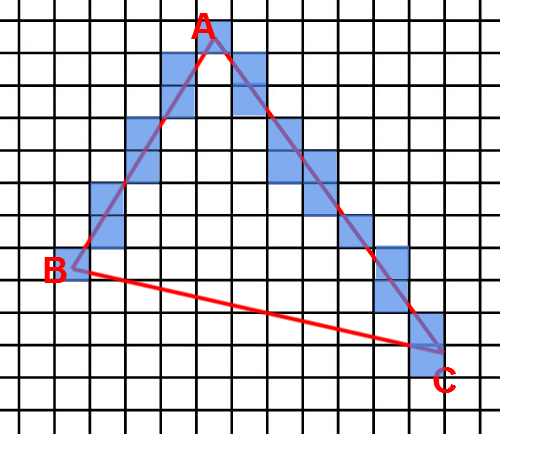
\includegraphics[width=0.4\linewidth]{rasterization_filledges}
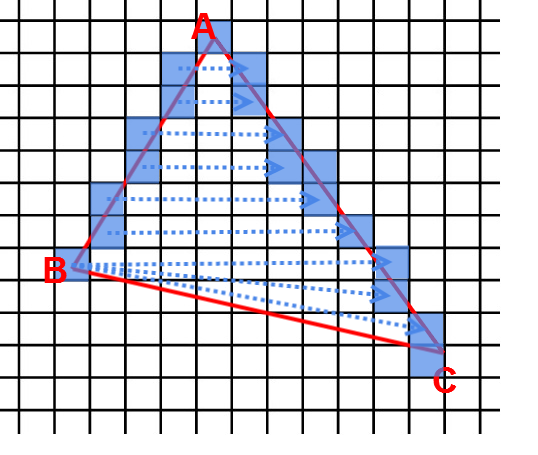
\includegraphics[width=0.4\linewidth]{rasterization_fillsurface}
\caption{Fill voxels on edges AB and AC. Then with the help of voxels on edges AB and AC, voxels inside the triangle can also be filled} \label{rasterization}
\end{figure}

To fill voxels between two vertices is not difficult. Firstly compute the normalized vector between these two vertices. Then start from one vertex and go along with the direction of the vector and fill voxels. The code is demonstrated as below:

%rasterization between two vertices
\begin{lstlisting}[xleftmargin=1em]
/* fill voxels(grid) between two vertices */
Vector v12 = point2-point1;
double len12 = v12.norm();
v12.normalise();

int n_points = 0;
for(unsigned int n=0;n<=floor(len12);n++)
{
    //go along with the direction of the vector and fill voxels
	Point temp_p;
	temp_p.x() = round(point1.x()+v12.x()*double(n));
	temp_p.y() = round(point1.y()+v12.y()*double(n));
	temp_p.z() = round(point1.z()+v12.z()*double(n));

	int grid_coordinate	= int(temp_p.x()*2*RADIUS*2*RADIUS + temp_p.y()*2*RADIUS + temp_p.z());

	//discard outliers
	if(grid_coordinate>(2*RADIUS*2*RADIUS*2*RADIUS-1) || grid_coordinate<0)  continue; 

	if(*(grid+grid_coordinate)!=true)
	{
		*(grid+grid_coordinate) = true;
		inter12.push_back(temp_p);
		grid_points.push_back(temp_p);
		n_points++;
	}
}

//fill the remaining voxels
int grid_coordinate_p2 = int(point2.x()*2*RADIUS*2*RADIUS + point2.y()*2*RADIUS + point2.z());
//make sure points in the range
if(grid_coordinate_p2<(2*RADIUS*2*RADIUS*2*RADIUS-1) && grid_coordinate_p2>0){
	if(*(grid+grid_coordinate_p2)!=true)
	{
		*(grid+grid_coordinate_p2) = true;
		inter12.push_back(point2);
		grid_points.push_back(point2);
		n_points++;
	} 
}
\end{lstlisting}

With $R = 32$, the size of the voxel grid is $2R\times2R\times2R = 262144$, which may occupy a huge memory space. So it is necessary to find a method, which can both save memory and compress the computational complexity. One approach is to create a temporary bitmap (bitset or boolean array in C++) of length $2R\times2R\times2R$ to record whether a voxel is filled. Each element of this bitmap can only show 1 or 0 (true or false), so that the whole bitmap will not occupy any redundant space. While in one traversal($O(n)$) of surfaces of the model, the voxel grid will be filled and the grid vertices should be stored. The peudocode shows this approach: 

%fill voxel grid
\begin{lstlisting}[xleftmargin=1em]
/* fill voxel grid and get rasterized points in O(n) */

bitmap = new bitmap(2R*2R*2R)               //temporary bitmap
for each voxel to be filled
    if(bitmap(voxel.x,voxel.y,voxel.z))==0  //has not been filled or registered
        bitmap(voxel.x,voxel.y,voxel.z)=1
        grid_point.push_back(voxel)
    end
end
delete bitmap;
\end{lstlisting}

The second pre-processing step is normalization. To normalize, the first step is to compute the center of mass. Then the average distance should be computed and the proportion of the average distance and $R$ can be acquired. Afterwards every vertex is scaled so that the average distance from voxels to the center of mass is $ \frac{R}{2}$. While normalizing, the center of mass will be moved to the origin. This helps further computation of spherical harmonics and distance histogram descriptors.

\section{Rotation Invariant Descriptors}

Both spherical harmonics descriptors and distance histogram descriptors are rotation invariant descriptors. So these two descriptors can be combined for retrieval. Before carrying out spherical harmonics transformation, the rasterized grid voxels should be transformed to polar coordinates as $f(r,\theta,\phi)$, and sorted according to their distances to the center of mass. A class for polar points is implemented. Its operator $<$ and $>$ are overloaded for suiting the STL sorting algorithm. 

As the radius range is from 0 to 32, the polar points can be devided and form a set ${\left\{ f_0,f_1,...,f_R \right\}}$, with 
\begin{equation}
f_r(\theta,\varphi)=f(r,\theta,\phi).
\end{equation}
Spherical harmonics decomposition can be applied for each $f_r(\theta,\phi)$, so that
\begin{equation}
f_r(\theta,\varphi)=\sum_{l=0}^{\infty}\sum_{m=-l}^{m=l}a_{lm}Y_{l}^{m}(\theta,\varphi),
\end{equation}
where
\begin{equation}
Y_\ell^m( \theta , \varphi ) = (-1)^m \sqrt{{(2\ell+1)\over 4\pi}{(\ell-m)!\over (\ell+m)!}} \, P_\ell^m ( \cos{\theta} ) \, e^{i m \varphi }.
\end{equation}
But the frequency $l$ goes to infinite. It is not able to implement. So it is restricted and a cutoff frequency is set as 32. The decomposition is 
\begin{equation}
f_r(\theta,\varphi)=\sum_{l=0}^{32}\sum_{m=-l}^{m=l}a_{lm}Y_{l}^{m}(\theta,\varphi).
\end{equation}

Details of spherical harmonics decomposition can be seen in Section~\ref{computational_techniques} Computational Techniques of Chapter~\ref{background} Background. For each frequency $l$ and each radius range $r$, the energy can be computed as the $L_{2}$-$norm$ of $a_{lm}$. Let $E_{lr}$ denote the energy in frequency $l$ and radius $r$, we have
\begin{equation}
E_{lr}=\sum_{m=-l}^{m=l}\|a_{ml}\|^{2}.
\end{equation}
The energy is rotation invariant. Therefore spherical harmonics descriptors $SH$ are able to acquire,
\begin{equation}
SH(l,r) = E_{lr}.
\end{equation}

Since with all the coefficients $a_{lm}$, the spherical function $f(\theta,\varphi)$ can perfectly reconstructed. Therefore, the energy of the sum of the coefficients $a_{lm}$ can represent the feature of the spherical function $f(\theta,\varphi)$. Moreover, the spherical harmonics $SH$ is the collection of the energies $E_{lr}$. Thus it can represent the shape feature of the 3D model. 

The pseudocode for spherical harmonics descriptors:

\begin{lstlisting}[xleftmargin=1em]
/* spherical harmonics descriptors */

for each frequency l
    for each rasterized vertex in one radius range r 
        calculate F_lr = F(l,r)
    end
    a_ml = sum of F_lr in one radius ragion
    SH(l,r) += abs(a_ml)^2    
end
SH = sqrt(SH)
\end{lstlisting}

The code for spherical harmonics descriptors:

\begin{lstlisting}[xleftmargin=1em]
/* spherical harmonics descriptors */

int idx_n = 0;
double *SH_descriptor;
SH_descriptor = new double [MAX_R*MAX_L]();

for(unsigned int idx_r = 1;idx_r<=RADIUS;idx_r++)
{
	//for each frequency
	for(int idx_l = 0;idx_l<MAX_L;idx_l++)
	{
		vector<double> 	a_ml_pow;
		//traverse frequency range
		for(int idx_m = -idx_l;idx_m<=idx_l;idx_m++)
		{
			vector<double> Yml_real,Yml_imag;
			double NPml;

			while(idx_n<=(grid_polar_points.size()-1) && grid_polar_points.at(idx_n).distance()<idx_r)
			{
				//initial Y_ml = N*P(m,l,cos(theta))*exp(i*m*phi)
				//function gsl_sf_legendre_sphPlm returns value of N*P(m,l,cos(theta))
				//cos(x) input should be a radian
				//theta_vector and phi_vector are radians
				PolarPoint current_p = grid_polar_points.at(idx_n);
				if(idx_m>=0)
				{
					NPml = gsl_sf_legendre_sphPlm(idx_l,idx_m,cos(current_p.theta()));
					Yml_real.push_back(NPml*cos(double(idx_m)*current_p.phi()));
					Yml_imag.push_back(NPml*sin(double(idx_m)*current_p.phi()));
				} else {
					NPml = pow (-1.0,-idx_m)*gsl_sf_legendre_sphPlm(idx_l,-idx_m,cos(current_p.theta()));
					Yml_real.push_back(NPml*cos(double(-idx_m)*current_p.phi()));
					Yml_imag.push_back(NPml*sin(double(-idx_m)*current_p.phi()));
				}
				idx_n++;
				if(idx_n==(grid_polar_points.size()-1)) break;
			}//while(dist_vector.at(idx_n)<idx_r)

			double 	a_ml_real,a_ml_imag;
			a_ml_real=accumulate(Yml_real.begin(),Yml_real.end(),0.0);
			a_ml_imag=accumulate(Yml_imag.begin(),Yml_imag.end(),0.0);
			a_ml_pow.push_back(pow(a_ml_real,2.0)+pow(a_ml_imag,2.0));
			if(idx_l!=MAX_L-1) idx_n-=Yml_real.size();
		}//finish traversing frequency range
		SH_descriptor[(idx_r-1)*MAX_R+idx_l] = sqrt(accumulate(a_ml_pow.begin(),a_ml_pow.end(),0.0));
	}
}

/*write out the data*/
WriteSH(write_filename,SH_descriptor);

delete [] SH_descriptor;
\end{lstlisting}

As for the distance histogram descriptors, they are simpler and are used to correct or supplement the spherical harmonics descriptors. First, the center of mass should be acquired. Then for each voxel in the grid, compute its distance to the center of mass. The distance within certain range will be recorded and counted. Lastly, the 
distribution of distances from vertices to the center of mass is acquired. This distribution is just the distance histogram descriptors.  

\section{Retrieval}

